#import "@local/bootlin:0.1.0": *

#import "@local/bootlin-yocto:0.1.0": *

#import "@local/bootlin-utils:0.1.0": *

#import "../../typst/local/themeBootlin.typ": *

#import "../../typst/local/common.typ": *

#show: bootlin-theme.with( aspect-ratio: "16-9", config-common(handout: "handout" in sys.inputs and sys.inputs.handout == "1", ))

#show raw.where(block: true): set block(fill: luma(240), inset: 1em, radius: 0.5em, width: 100\%)

#show raw.where(block: true): set text(size: 11pt)

#show raw.where(block: false): r => text(fill: color-link)[#r]

#show raw.where(lang: "c", block: true): set block(fill: luma(240), inset: 0.4em, radius: 0.5em, width: 95\%, breakable: true, above: 12pt, below: 12pt)

#show raw.where(lang: "c", block: true): set text(11pt)

#show raw.where(lang: "console", block: true):set block(fill: luma(240), inset: 0.4em, radius: 0.5em, width: 95\%, breakable: true, above: 6pt)

#show raw.where(lang:"console", block: true): set text(12pt)

=== Time your commands using the time command
\begin{center}
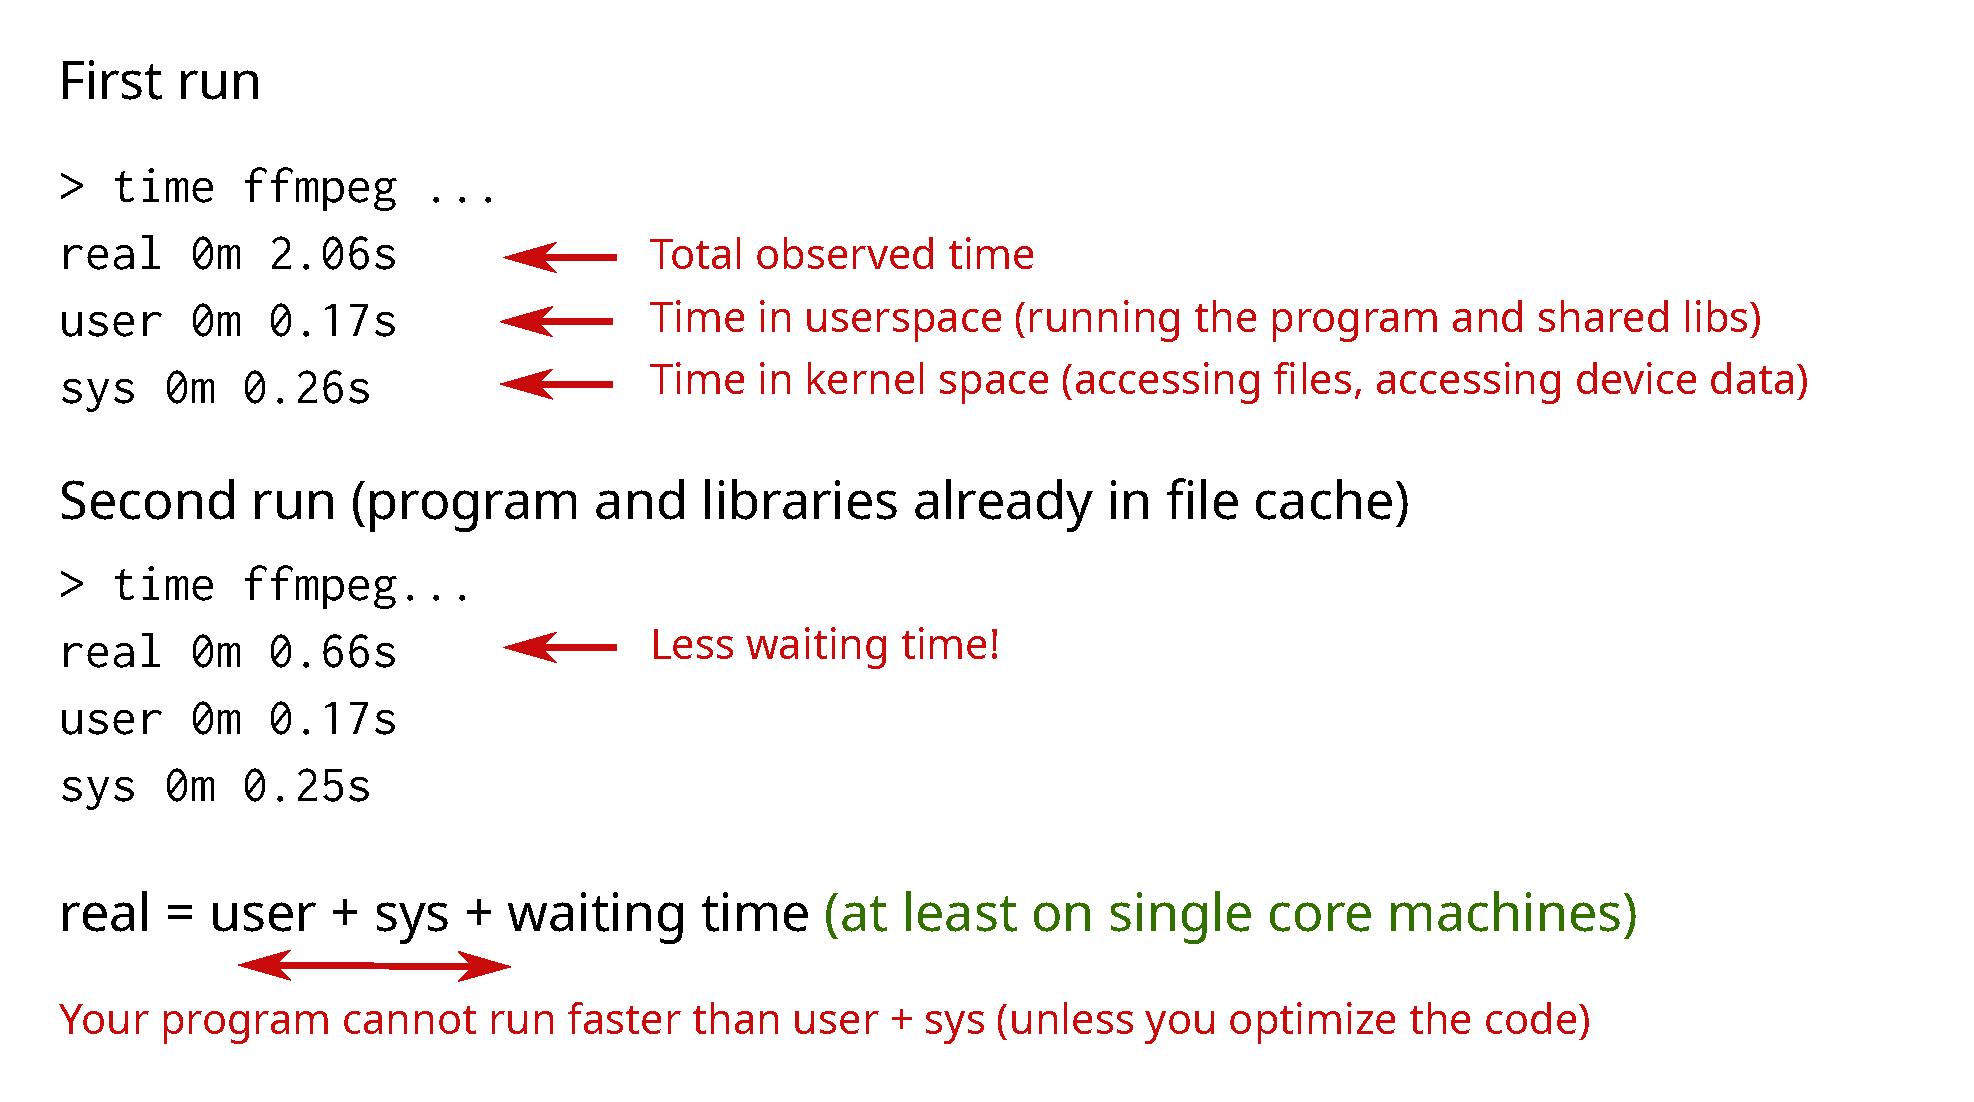
\includegraphics[height=0.7\textheight]{slides/boot-time-toolchain2/using-time-command.pdf}
\end{center}
This gives you the best time that can possibly be achieved (with the fastest storage).


#setuplabframe([Toolchain optimizations],[
\begin{itemize}
\item Measure filesystem and `ffmpeg` binary size. Time
      the execution of the application.
\item Re-compile the root filesystem using a Thumb2 toolchain
\item Re-compile the root filesystem with the {\em Musl}
      C library instead of {\em uClibc}
\item Find the best toolchain in terms of size and execution time.
\item Have Buildroot generate an external toolchain ({\em SDK})
\end{itemize}
])


=== Lessons from labs: ARM vs Thumb2 (32 bit only)
\begin{itemize}
\item Testcase: root filesystem with `ffmpeg` and associated
      libraries (from our training labs), with uClibc
\item Compiled with gcc 10.3, generating {\em ARM} code:\\
      Total filesystem size: 17.9 MB\\
      `ffmpeg` size: 239 KB
\item Compiled with gcc 10.3, generating {\em Thumb2} code:\\
      Total filesystem size: 14.5 MB (-19 \%)\\
      `ffmpeg` size: 191 KB (-20 \%)
\item Performance aspect: performance apparently slightly improved with Thumb2
      (about 2 \%, but there are slight variations in measured
      execution time, for one run to another).
\end{itemize}


=== Lessons from labs: musl vs uClibc Replacing {\em uClibc} by {\em musl} in our video player lab, keeping
{\em Thumb2}. Here are data from an earlier run of our labs:
\begin{itemize}
   \item Total system size with {\em uClibc}: 14.3 MB
   \item Total system size with {\em Musl}: 14.4 MB
   \item uClibc saves 80 KB (useful), but otherwise no other significant change
    in filesystem and code size. Not a surprise when the system is mostly filled
    with binaries relying on shared libraries.
\end{itemize}
Switching to {\em Musl} as it is supposed to allow for smaller static binaries, which will be useful in later labs.

